

\section{Adaptación de la metodología}

 A continuación se presenta la forma en que ha sido configurado el marco de trabajo {\it Scrum}
 para trabajar en concordancia con los marcos de trabajo {\it Octalysis} y {\it For The Win}
 usados cómo guía para la diseño de los componentes creados para la implementación de
 Gamificación en una plataforma en línea.

\subsection{Roles}

 \noindent 
 El marco de trabajo {\it Scrum} define los roles: scrum master, dueño del producto, stakeholders,
 y equipo de desarrollo. A continuación se especifica las personas que estarán cumpliendo los
 distintos roles en Scrum.

\subsubsection{Product Owner}

 Durante este proyecto el rol del dueño del producto (o {\it product owner}) lo llevarán a cabo
 los directores del trabajo terminal, ya que son a máxima autoridad entorno a la definición del
 alcance, ambos directores son listados a continuación:

    \begin{quote}
    \begin{itemize}
        \item {\it M. en C.} Sandra Ivette Bautista
        \item {\it M. en C.} Edgar Armando Catalán Salgado
    \end{itemize}
    \end{quote}

 \noindent 
 A pesar de que en la guía oficial de scrum \cite{TheScrumGuide} se especifica que el {\it
 product owner} debe ser una persona, se decidió que este rol fuera llevado acabo mediante los
 directores del trabajo terminal, con la presima de que para la toma de decisiones ambos
 directores deben estár de acuerdo.

\subsubsection{Equipo de desarrollo}

 Durante este trabajo el equipo de desarrollo estará conformado por un total de
 tres integrantes, siento estos los alumnos que presentan el trabajo terminal. Los miembros del
 equipo de desarrollo team son listados a continuación:

    \begin{quote}
    \begin{itemize}
        \item David Flores Casanova
        \item Ricardo Naranjo Polit
        \item Daniel Isaí Ortega Zúñiga
    \end{itemize}
    \end{quote}

% ROLES - PRODUCT OWNER

 % \noindent
 % Para que las funciones del Product Owner sean exitosas, la organización debe respetar sus
 % decisiones. Nadie puede forzar al Development Team para trabajar en un conjunto distinto
 % de requerimientos establecidos en el Product Backlog.

% ROLES - EQUIPO DE DESARROLLO

 % durante el desarrollo de este proyecto el equipo de desarrollo estará conformado por:

 % \noindent El tamaño del equipo debe ser lo suficientemente pequeño para permanecer ágil y lo
 % suficientemente grande para realizar entregas significativas al final de cada {\em Sprint}.\\
 % Un equipo con menos de tres miembros disminuiría la interacción y por lo tanto la productividad,
 % por otro lado, con más de nueve miembros se requiere mayor coordinación con más complejidad.

\subsubsection{Maestro Scrum}

 El rol del {\it Scrum Master} durante este proyecto se llevará a cabo mediante
 dos personas con la finalidad de dividir las responsabilidades y no sobrecargar de trabajo
 a una persona. El {\it Scrum Master} estará conformado por:

    \begin{quote}
    \begin{itemize}
        \item M. en C. Edgar Armando Catalán {\it (Responsabilidades hacia el Product Owner)}
        \item Daniel Isaí Ortega {\it(Responsabilidades hacia el equipo de desarrollo)}
    \end{itemize}                        
    \end{quote}


\subsubsection{Stakeholders}

 Los Stakeholders son personas externas al equipo Scrum con un interés y/o conocimientos
 específicos del producto \cite{ScrumGlosary}. En relación a la naturaleza del proyecto se
 considera a los sinodales cómo los Stakeholders oficiales, los cuales son listados a
 continuación:

    \begin{quote}
    \begin{itemize}
        \item Dra. Fabiola Ocampo Botello
        \item M. en C. María del Socorro Téllez Reyes
        \item M. en C. José David Ortega Pacheco
    \end{itemize}
    \end{quote}

\subsection{Eventos}
 
 A continuación se detalla cómo han sido configurados los distintos eventos dentro del marco de trabajo
 Scrum, los cuales contemplan las iteraciones o los {\it Sprints}, reuniónes diarias, las etapas de
 planeación, revisión y retroalimentación.

\subsubsection{Sprints}

 \noindent Para este proyecto los Sprints están configurados a una duración de 14 días con una
 estimación de 18 iteraciones, la duración de dos semanas se estableció con el propósito de:
    
    \begin{itemize}
    \item Incrementar la retroalimentación y detectar los impedimentos
          en la forma de trabajo lo más pronto posible, y

    \item Realizar incrementos más cortos y continuos considerando que el
          equipo de desarrollo está conformado por tres integrantes.
    \end{itemize}

 \noindent 
 La figura \ref{tbl:sprints}, mostrada en la siguiente página, representa una estimación de fueron
 organizados los {\it sprints} a lo largo del proyecto. La primer etapa de {\bf investigación
 y analisis general} contiene forma de trabajo, la investigación acerca de la gamificación en la educación
 y finalmente la definición del alcance general. Posteriormente cada dos sprints se llevan a cabo las {\bf
 etapas de analisis, diseño, desarrollo y pruebas para cada módulo}. \clearpage

    \begin{sidewaysfigure}
        \centering
        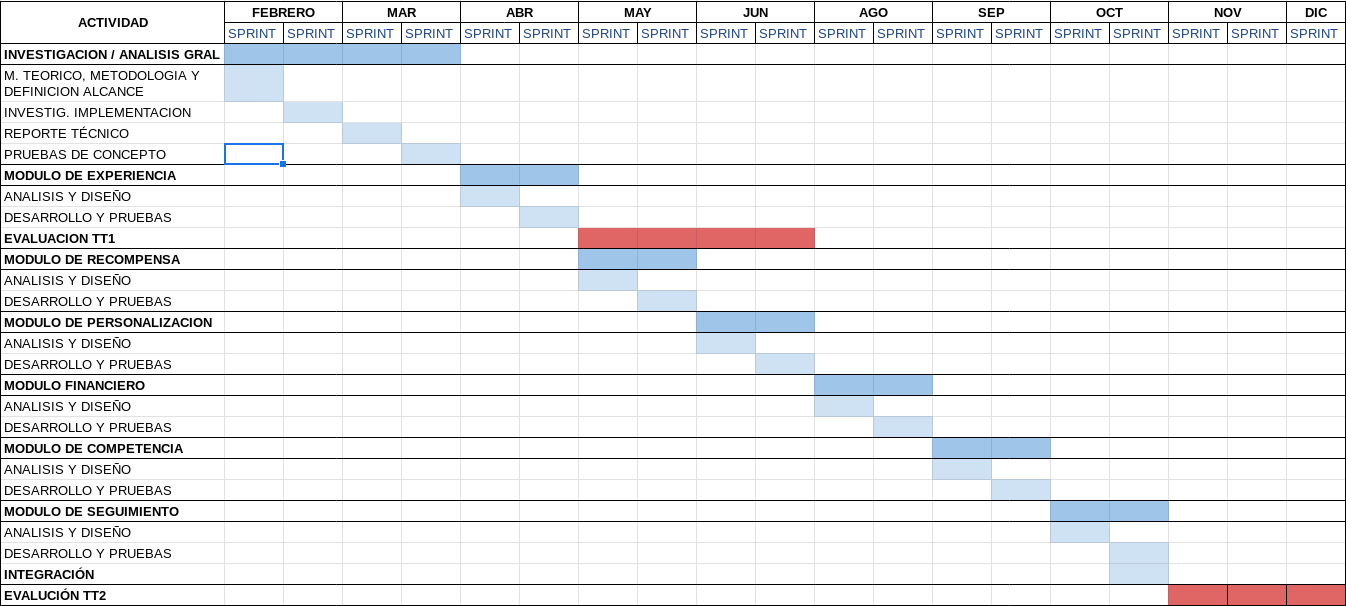
\includegraphics[width=1\textwidth]{analisis/diagrams/cronograma}
        \caption{Cronograma de actividades}
        \label{fig:awesome_image}
    \end{sidewaysfigure}

 \clearpage

    {\centering\color{primary}\Huge THIS PAGE SHOULD BE REMOVED}

    \addtable{|c|c|c|l|}{tbl:sprints}{
        {\bf No Sprint} & {\bf Fecha Inicio} & {\bf Fecha Final}  & {\bf Tarea}\\\hline
        
        1  &  5 de Febrero    & 18 de Febrero    & Marco Teórico, Metodología, Definición del Alcance \\\hline
        2  & 19 de Febrero    &  4 de Marzo      & Investigación de Implementación \\\hline
        3  &  5 de Marzo      & 18 de Marzo      & Reporte Técnico del Trabajo Terminal \\\hline
        4  & 19 de Marzo      &  1 de Abril      & Pruebas de Concepto\\\hline

        \rowcolor{orange}
        5  &  2 de Abril      & 15 de Abril      & Mod. Experiencia: análisis y diseño \\\hline
        6  & 16 de Abril      & 29 de Abril      & Mod. Experiencia: desarrollo y pruebas\\\hline
        
        7  & 30 de Abril      & 13 de Mayo       & Mod. Recompensa: análisis y diseño \\\hline
        8  & 14 de Mayo       & 27 de Mayo       & Mod. Recompensa: desarrollo y pruebas \\\hline
        
        9  & 28 de Mayo       & 10 de Junio      & Mod. Personalización: analisis y diseño\\\hline % FIN SEMESTRE
        10 & 11 de Junio      & 24 de Junio      & Mod. Personalización: desarrollo y pruebas \\\hline
        
        11 & 25 de Junio      &  8 de Julio      & Mod. Financiero: analisis y diseño \\\hline
        12 &  9 de Julio      & 22 de Julio      & Mod. Financiero: desarrollo y pruebas \\\hline

        13 & 23 de Julio      &  5 de Agosto     & Mod. Competencia: analisis y diseño \\\hline % INICIO SEMESTRE
        14 &  6 de Agosto     & 19 de Agosto     & Mod. Competencia: desarrollo y pruebas \\\hline
        
        15 & 20 de Agosto     &  2 de Septiembre & Mod. Seguimiento: analisis y diseño \\\hline
        \rowcolor{green}
        16 &  3 de Septiembre & 16 de Septiembre & Mod. Seguimiento: desarrollo y pruebas \\\hline
        
        17 & 17 de Septiembre & 30 de Septiembre & Pruebas de Integración\\\hline
        18 &  1 de Octubre    & 14 de Octubre    & Caso de Estudio I (y correcciones)\\\hline
        19 & 15 de Octubre    & 28 de Octubre    & Caso de Estudio II \\\hline
        
        %20 & 29 de Octubre    & 17 de Noviembre  & Pruebas de Integración\\\hline
        %21 & 18 de Noviembre  & 25 de Noviembre  & Ejecución del Caso de Estudio\\\hline
        %22 & 26 de Noviembre  &  9 de Diciembre  & ''\\\hline % FIN DE SEMESTRE
        
    }{Detalle de Sprints (Estimación)}

 \clearpage

\subsubsection{Planeación}

 \noindent El día acordado para llevar a cabo esta reunión fueron los {\bf martes} cada dos semanas
 {\bf a la 1:30pm} en las instalaciones de la Escuela Superior de Cómputo (ESCOM). El horario fue
 acordado tomando en cuenta la disponibilidad de todos los miembros del equipo Scrum.
    
    \begin{quote}
    {\bf Nota:} En caso de que, por algun evento extraordinario, no se pueda
                llevar a cabo la etapa de planeación esta reunión se reagendará
                para que ocurra lo más pronto posible.
    \end{quote}

\subsubsection{Reunión diaria}

 \noindent 
 Para llevar a cabo las reuniones diarias se establecieron por defecto días, lugar y hora detallados
 en la tabla \ref{tbl:daily}. Esta reunión sera realizada entre los miembros del equipo de desarrollo
 debido a la dificultad de hacer coincidir los horarios del equipo de desarrollo con los del {\it Product
 Owner}.

    \addtable{|c|c|c|}{tbl:daily}{
       {\bf Día de Trabajo} & {\bf Lugar} & {\bf Hora Inicio} \\\hline
       Lunes     & ESCOM Sala 21 N & 10:00am \\\hline
       Martes    & ESCOM Sala 21 N & 10:00am \\\hline
       Miércoles & ESCOM Sala 21 N & 10:00am \\\hline
       Jueves    & ESCOM Sala 21 N & 10:00am \\\hline
       Viernes   & ESCOM Sala 21 N & 10:00am \\\hline
       Domingo   & -               & 12:00pm \\\hline
    }{Horario y lugar acordado de las reuniones diarias}

    \begin{quote}
    Los días domingos la reunión diaría se llevará a cabo a traves de una llamada grupal
    entre los miembros del equipo de desarrollo.
    \end{quote}

\subsubsection{Revisión}

 \noindent Debido a que en este proyecto, los stakeholders y el equipo de scrum tienen distintos horarios
 de disponibilidad, la revisión del {\it sprint} se divide en cuatro fases, aplicando la primer fase a los sprints
 impares y las cuatro fases para sprints pares. Las fases de describen a continuación:
 
    \begin{quote}
    \begin{itemize}
    \item[\it Fase 1]
        Consiste en realizar una primer reunión con el equipo scrum para obtener una
        retroalimentación y revisar el incremento entregado.

    \item[\it Fase 2]
        En esta fase el equipo de desarrollo tiene reuniones con los Stakeholders con la
        finalidad de obtener retroalimentación y observaciones acerca de la forma de
        trabajo y del incremento.

    \item[\it Fase 3] 
        En esta fase los miembros del equipo scrum revisarán las observaciones y
        comentarios de los {\it Stakeholders} para saber cuales proceden.

    \item[\it Fase 4]
        Se avisa a los Stakeholders acerca de cuales observaciones procedieron y cuales no.\\
    \end{itemize}    
    
    {\bf Nota:} Las reuniones de la fase 2, dependen de la disponibilidad que cada {\it stakeholder} tenga,
                en caso de que ningún stakeholder tenga disponibilidad para llevar a cabo la fase 2,
                el proceso de la revisión del {\it Sprint} terminará.
    \end{quote}

 \noindent \message{^^JWarning WE DONT RESPECT THE STABLISHED SPRINT REVIEW pp.\thepage}

\subsubsection{Retroalimentación}

 \noindent La etapa de retroalimentación consiste en una reunión interna para discutir aquellas cosas que han
 sucedido correctamente y cuales deben mejorar. Esta reunión se realizará al final de cada {\it Sprint} estando
 presentes los directores del trabajo terminal y los miembros del equipo de desarrollo.

\subsection{Artefactos}

 \noindent
 A continuación se describe la forma en que serán se llevarán a cabo los artefactos definidos por el marco
 de trabajo Scrum, además se describe los atributos con los que serán especificados los elementos del
 {\it Product Backlog} y {\it Sprint Backlog}.

\subsubsection{Product Backlog}

 \noindent Debido a que el proyecto requería una etapa de investigación, se optó por tener dos tipos
 de {\it items} en el product backlog, los items de documentación/preparación del proyecto  y los {\it items}
 para desarrollo del mismo.\\
    
 \noindent{\bf Items de Documentación}\\
 Los items de preparación del proyecto y documentación deben ser especificados
 mediante los atributos presentes en la tabla \ref{attrPBpre}:
    
    \addtable{|l|l|}{attrPBpre}{
        {\bf Atributo} & {\bf Descripción}                                                             \\\hline
        id           &  Es una identificador de la forma ``Ax'' donde {\it x} es un número consecutivo \\\hline
        nombre       &  Nombre representativo de la actividad                                          \\\hline
        descripción  &  Detalle de lo que hay que hacer para llevar a cabo esta actividad.             \\\hline
        sprint       &  Indica el número de Sprint al cual ha sido asignada esta tarea.                \\\hline
        %estado      & Indica el estado ({\it por hacer, en proceso o concluida} de una actividad. \\\hline
        %estimación  & Especifica el periodo de tiempo estimado para la liberación de dicha actividad. \\\hline
    }{Atributos de los Items del P.B de Documentación}


 \noindent{\bf Items de Desarrollo del Proyecto}\\
 Describen las características del software que se desarrollará, estos items deben
 ser redactados de manera objetiva y como requerimientos del sistema, y deben contener
 los atributos presentes en la tabla \ref{attrPB}:
    
    \addtable{|l|p{0.62\textwidth}|}{attrPB}{
        {\bf Atributo} & {\bf Descripción}\\\hline
        id           &  Es una identificador de la forma '{\bf RFx}' o '{\bf RNFx}' para requerimientos    \par
                        funcionales y no funcionales respectivamente. {\it x} es un número consecutivo     \\\hline

        nombre       &  Nombre representativo del requerimiento del sistema.                               \\\hline
        descripción  &  Descripción concisa y objetiva acerca del requerimiento.                           \\\hline
        prioridad    &  Indica la prioridad de un requerimiento, los valores posibles son:                 \par
                        \qquad MA (muy alta), A (alta), M (Media), B (baja) y MB (muy baja)                \\\hline

        sprint       &  Indica el número de Sprint al cual ha sido asignado este requerimiento.            \\\hline
        tipo         &  Tipo de requerimiento no funcional según la clasificación propuesta por Frank Tsui \\\hline
        %estimación  & Especifica el periodo de tiempo estimado para la liberación de dicho requerimiento. \\\hline
 }{Atributos de los Items del P.B de Desarrollo del Proyecto}
  
 \begin{quote}
 {\bf Nota:} El atributo {\it Sprint} debe estar presente en todos los items correspondientes
              al sprint corriente y a los sprints anteriores a este. El atributo {\it Sprint}
              puede no estar presente en los items que no han sido vinculados a un Sprint. 
 \end{quote}
 
\subsubsection{Sprint Backlog}

 \noindent Conforme los {\it items} del {\it product backlog} vayan siendo seleccionados para
 tratarse en un sprint, se les añadirá los atributos presentes en la tabla \ref{SBItems}, los
 cuales son una etiqueta que indique a qué sprint pertenecen y opcionalmente una etiqueta que
 indique cómo se evaluará la completitud de dicho item.
    
    \addtable{|l|l|}{SBItems}{
        {\bf Atributo} & {\bf Descripción}\\\hline
        sprint   &  Indica el número de Sprint al cual ha sido asignado el item.             \\\hline
        pruebas  &  (Opcional) Sentencia de cómo se evaluara que dicho ítem esté completado. \\\hline

    }{Atributos del Sprint Backlog}

% ======================================================
%   F O R   T H E   W I N
% ======================================================

\section{Marco de Trabajo For The Win}
\label{analisis:forthewin}

 Una de las herramientas más importantes que brinda el marco de trabajo {\it For The Win} es
 una guía pragmática para la implementación de la gamificación, dicha guía consiste de seís
 pasos, el detalle de cómo se siguieron estos pasos se encuentra en las siguientes secciones
 de este capítulo de análisis.

    \begin{quote}
    \begin{itemize}
    \item El primer paso del marco de trabajo consiste en definir los objetivos del
          sistema, mientras que el segundo consiste en delimitar las acciones de los
          usuarios, especificando el comportamiento que tendrán dentro del sistema.
          Ambos puntos son tratados en la siguiente sección \hyperrefx{analisis:modulos}.\\

    \item El siguiente paso consiste en definir que usuarios interactuarán con el sistema
          y construir las funcionalidades con base en los tipos de usuarios que lo
          usarán, para ello se destina la sección \hyperrefx{analisis:usuarios}.\\

    \item El cuarto paso del marco de trabajo consiste en definir los ciclos de actividades
          o las etapas por las que pasa un usuario para avanzar en el sistema gamificado.
          Para este punto se presenta en la sección \hyperrefx{analisis:visionyuso}.\\

    \item El quinto paso tiene el titulo {\it``Piensa en la diversión''}, de acuerdo con el
          marco de trabajo para poder solventar este punto el diseño de los elementos de
          juego debe contemplar tanto elementos que apoyen a la motivación extrínseca cómo
          a la motivación intrínseca. El mapeo entre los módulos planteados y el tipo de
          motivación a la que brindan soporte se puede ver en la sección
          \hyperrefx{analisis:octalysis}.\\

    \item El último paso consiste en escoger especificamente que elementos de juego se
          deciden utilizar en el diseño del sistema, probarlos, ajustarlos y ejecutar
          los cambios requeridos para mejorar la implementación. Esta punto es tratado en
          parte del documento destinada a los módulos.
    \end{itemize}
    \end{quote}



